\section{Data set and analysis methods}
\label{sec:org65db251}
\subsection{The \(Y \rightarrow XX\)channel}
\label{sec:org0fd1492}
The \(Y \rightarrow XX\) dataset is composed of simulated events that represent the generic process of a resonance Y decaying into an XX pair, in the mass range between 100 and 300 GeV. The background consists of 50,839 events, while the signal comprises 5,946 events. The particular set is made up of miscellaneous pre-existing Monte Carlo (MC) samples, and the selected events contain only leptonic final states (one lepton and one antilepton of the same flavor). For the purpose of this study, only generator-level events were used, and given that we are not interested in any particular process, but rather in the most general case, no kinematic constraints were placed in the event selection. It should be noted that despite the fact that the parent MC samples contain lepton pairs in the final states, the resulting set can represent any diobject production in the selected mass range. The following table summarizes the features of the dataset in question:

\begin{table}[h!]
\centering
\begin{tabular}{ |p{3cm}|p{10cm}|  }
 \hline
Feature & Description \\
 \hline
$Pt_{1}$ &  The transverse momentum of the first particle in the XX pair \\
 \hline
$\eta_{1}$ &  The psudorapidity of the first particle in the XX pair \\
 \hline
$\phi_{1}$ &   azimuth angle of the first particle in the XX pair \\
 \hline
$Pt_{2}$ &  The transverse momentum of the second particle in the XX pair \\
 \hline
$\eta_{2}$ &  The psudorapidity of the second particle in the XX pair \\
 \hline
$\phi_{2}$ &   azimuth angle of the second particle in the XX pair \\
 \hline
\end{tabular}
\caption{Summary of the data set features }
\label{table:DataSetFeatures}
\end{table}

The mass spectrum for the \(Y \rightarrow XX\) decay, can be seen in figure \ref{fig:diX}

\begin{figure}[h!]
\centering
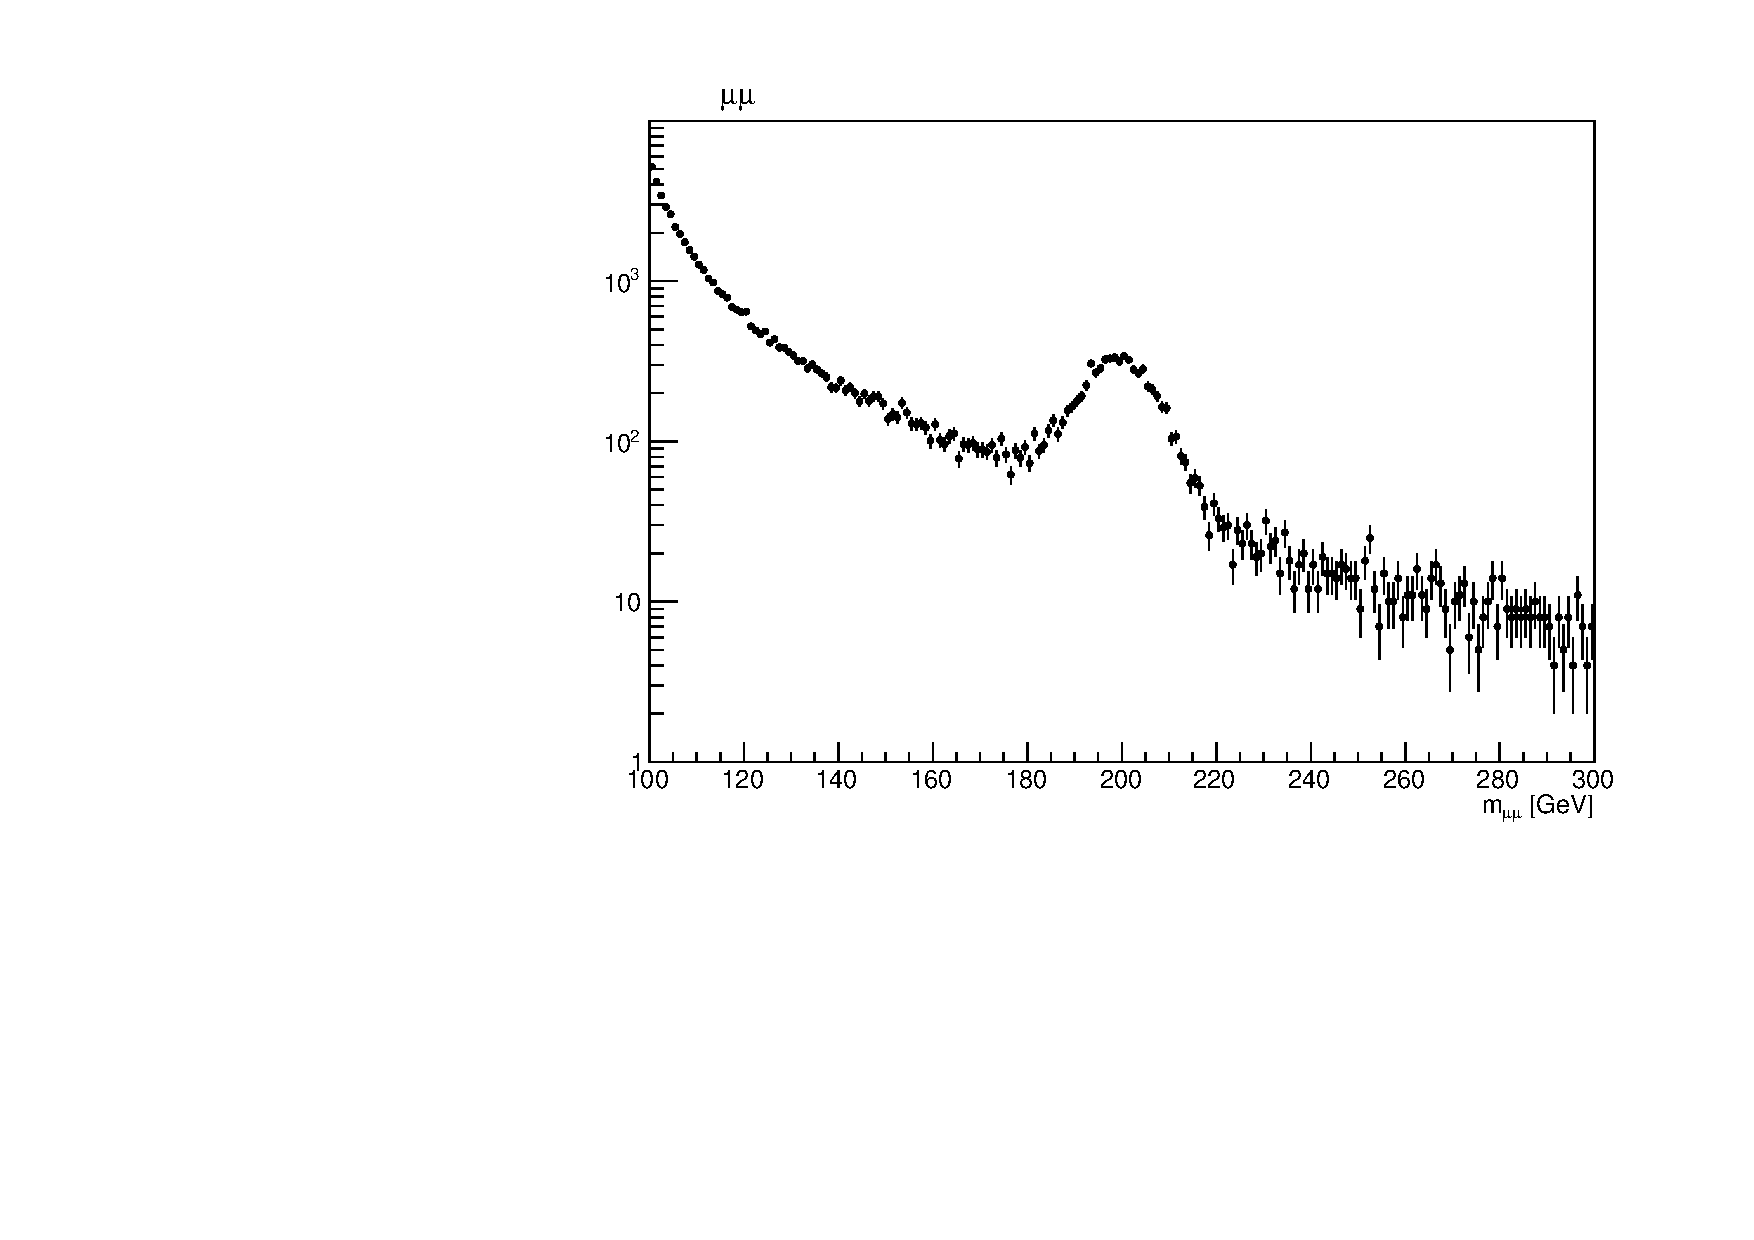
\includegraphics[width=0.5 \textwidth]{/home/kpapad/UG_thesis/Thesis/Analysis/out/Plots/DYJets_test2.pdf}
\caption{The $Y\rightarrow XX$ invariant mass spectrum}
\label{fig:diX}
\end{figure}

\subsection{Energy scale uncertainties}
\label{sec:org6831a0b}
Energy scale uncertainties have an effect on the transverse momenta \(P_t\) of the produced \(XX\) pair. Such uncertainties are modeled as random noise (Gaussian smearing) to the signal component. To smear the data by \(x\%\), we iterate over every signal event and multiply the transverse momenta by numbers sampled from a Gaussian distribution of \(\mu = 1\) and \(\sigma = x/100\), where \(x\) is the percentage of smearing (each \(P_t\) is multiplied by a different number).

In the present study, we compare the performance of a Boosted Decision Tree (BDT)-based analysis and a fit-based analysis on a given dataset for various cases of smearing (various values of \(\sigma\)). Table \ref{table:Smearings} summarizes the smearing percentages used for this analysis. The values are chosen such that we examine both cases of mild noise (\(0-5\%\)) up to extreme noise (\(50\%\)). Nevertheless, it should be noted that what is considered as an extreme case or a mild case of smearing is not defined in an absolute manner but rather is related to the mass range of the data upon which the blur is applied.

\begin{table}[h!]
\centering
\begin{tabular}{ |c|  }
 \hline
Percentage of smearing \\
 \hline
$0\%$\\
$5\%$\\
$10\%$\\
$15\%$\\
$20\%$\\
$30\%$\\
$40\%$\\
$50\%$\\
\hline
\end{tabular}
\caption{Summary of the smearing cases that will be studied in this work }
\label{table:Smearings}
\end{table}

\subsection{Statistical Interpretation of the results}
\label{sec:org1331983}
Usually, once the signal is separated from the background, a specific region is defined (either a BDT score range in case of a BDT-based analysis or a mass range in case of a fit-based analysis), and only the signal and background events falling within the defined region are selected. The question that arises is whether the selected signal is simply a statistical fluctuation of the background or not. In other words, how statistically significant is the signal? Because measurements at CMS are Poissonian in nature, the measured signal is compared to the Poissonian deviation of the background. Therefore, the significance we are interested in is defined as follows:
\begin{equation}
\text{Significance} = \frac{Signal}{\sqrt{Background}}
\end{equation}
Were signal and background signify the ammonut of signal and background events present in a the selected region.  
\subsection{Analysis Method I: Training a BDT Classifier}
\label{sec:org2ab78e2}
\subsubsection{The Train/Test/Application data sets}
\label{sec:orgbf7e2cb}
For the BDT training (and due to the lack of an infinite number of events), the original dataset had to be split into three parts. The training set is used to train the classifier. As the reader may have noticed, the signal events in the original dataset are much less than the background events. This class imbalance makes the training of the model much harder, and for that reason, the training set has been enriched with more (unseen) signal events, so that the two classes have the same number of events. The testing set is used to evaluate the training. For that purpose, the two signal and background classes also have the same number of events. Finally, the application set is used for the analysis. Through trial and error, we noticed that working with smaller statistics enhances the magnitude of statistical fluctuations in the analysis. To avoid such confusion, the application set contains a part of the testing set as well. This doesn't interfere with the training, since the BDT has never seen the testing events during training. Finally, it should be mentioned that in order to have an "apples-to-apples" comparison between the BDT-based analysis and the Fit-based analysis, the application set will be analyzed in both cases. For that reason, the smearing cases that will be discussed for the rest of this chapter will concern the application set.

Table \ref{table:TrainTestApp} summarizes the number of events used in each dataset.

\begin{table}[h!]
\centering
\begin{tabular}{ |p{3cm}|p{3cm}|p{4cm}|  }
 \hline
Data Set & No.Signal Events & No. Background Events \\
 \hline
Training & 3882 & 3882 \\
Testing & 3881 & 3881 \\
Application & 2973 & 20827 \\
 \hline
\end{tabular}
\caption{Sumarry of the Train Test Application number of events}
\label{table:TrainTestApp}
\end{table}
\subsubsection{Training}
\label{sec:orgf9d881c}
One of the key aspects of a successful training is the feature space that is being used. Although the Train/Test sets consist of the features described in Table \ref{table:DataSetFeatures}, those features are not optimal for the particular classification problem. The feature space that is found to be optimal for the problem in question consists of five features and is summarized in Table \ref{table:TrainFeatures} and Figure \ref{fig:TrainFeaturesPlot}.

\begin{table}[h!]
\centering
\begin{tabular}{ |p{3.5cm}|p{11cm}| }
 \hline
Feature & Description \\
 \hline
$Pt_{1}$ &  the transverse momentum of the first particle in the XX pair. \\
 \hline
$Pt_{2}$ &the transverse momentum of the second particle in the XX pair. \\
 \hline
$\Delta\phi = \phi_{2} - \phi_{1}$ & the difference in the azimuthal angles between the two particles in the XX pair. \\
 \hline
$\Delta\eta = \eta_{2} - \eta_{1}$ & the difference in the pseudorapidity values between the two particles in the XX pair. \\
 \hline
$\Delta R = \sqrt{\Delta\eta^{2} + \Delta\phi^{2}}$ & the separation in the eta-phi plane between the two particles in the XX pair. \\
 \hline
\end{tabular}
\caption{Sumarry of the features used for training }
\label{table:TrainFeatures}
\end{table}

\begin{figure}[h!]
\centering
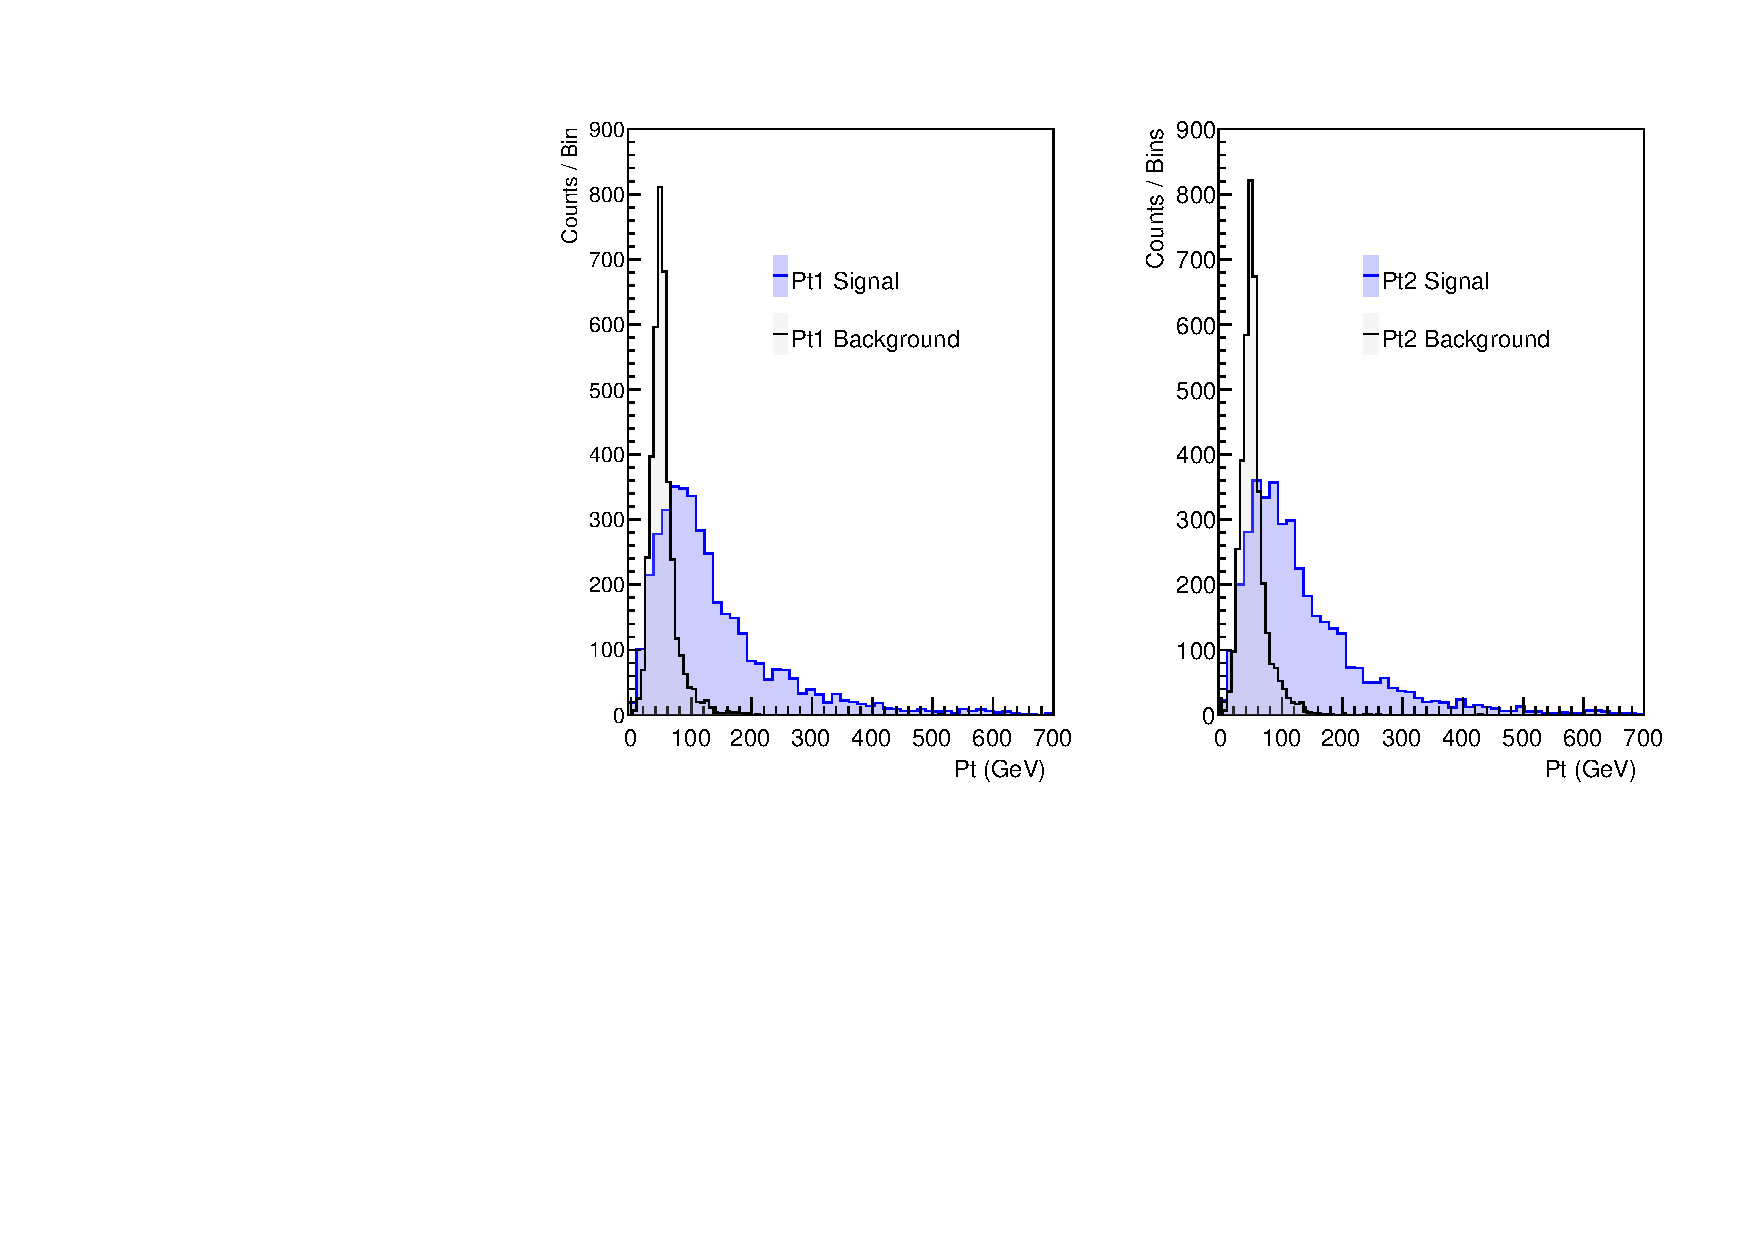
\includegraphics[page=1,width=0.6\textwidth]{/home/kpapad/UG_thesis/Thesis/Analysis/out/Plots/WPhiJets_M200M100300Deltas_varsplot.pdf}
\includegraphics[page=2,width=0.6\textwidth]{/home/kpapad/UG_thesis/Thesis/Analysis/out/Plots/WPhiJets_M200M100300Deltas_varsplot.pdf}
\caption{Sumarry of the features used for training }
\label{fig:TrainFeaturesPlot}
\end{figure}

To assess the performance of the trained model, the Area Under the Receiver Operating Curve (ROC-AUC) is used as a metric. However, it is important to note that in addition to evaluating the model's performance, we also consider the possibility of overfitting. To quantify overfitting, we examine the ratio of the number of training events to the number of testing events at a particular BDT score. If the model is not overtrained, the performance on the training and testing set will be approximately the same, and therefore, the ratio will fluctuate around 1 across the BDT score range.

Figure \ref{fig:BDTplot} displays the BDT score plot of the training and testing set, as well as the corresponding ROC curves. The performance of the model on the testing set yields an AUC score of 0.98. Looking at the Training/Testing ratios, one can notice that they fluctuate around one. The absence of a profound trend in both signal and background ratios implies that the model is not severely overfitted.
\begin{figure}[h!]
\centering
\begin{subfigure}{0.49\textwidth}
\centering
\includegraphics[page=5, width=\linewidth]{/home/kpapad/UG_thesis/Thesis/Bdt/out/Plots/WPhiJets_M200M100300DeltasPConf12BDTplot.pdf}
\caption{}
\end{subfigure}
\begin{subfigure}{0.49\textwidth}
\centering
\includegraphics[page=3, width=\linewidth]{/home/kpapad/UG_thesis/Thesis/Bdt/out/Plots/WPhiJets_M200M100300DeltasPConf12BDTplot.pdf}
\caption{}
\end{subfigure}
\caption{A: The BDT score of the Testing and Training sets. B: The roc curves for the training and testing sets}
\label{fig:BDTplot}
\end{figure}

\subsubsection{Application}
\label{sec:orgc469879}
The application of the model to the application set is a rather straightforward process. The data are simply "fed" to the model, and the latter performs the classification. The ROC curves for the performance of the trained model on the data for each of the smearing cases of table \ref{table:Smearings} are illustrated in figure \ref{subfig:SmearingROC}.

\begin{figure}[h!]
\centering
\begin{subfigure}{0.49\textwidth}
\centering
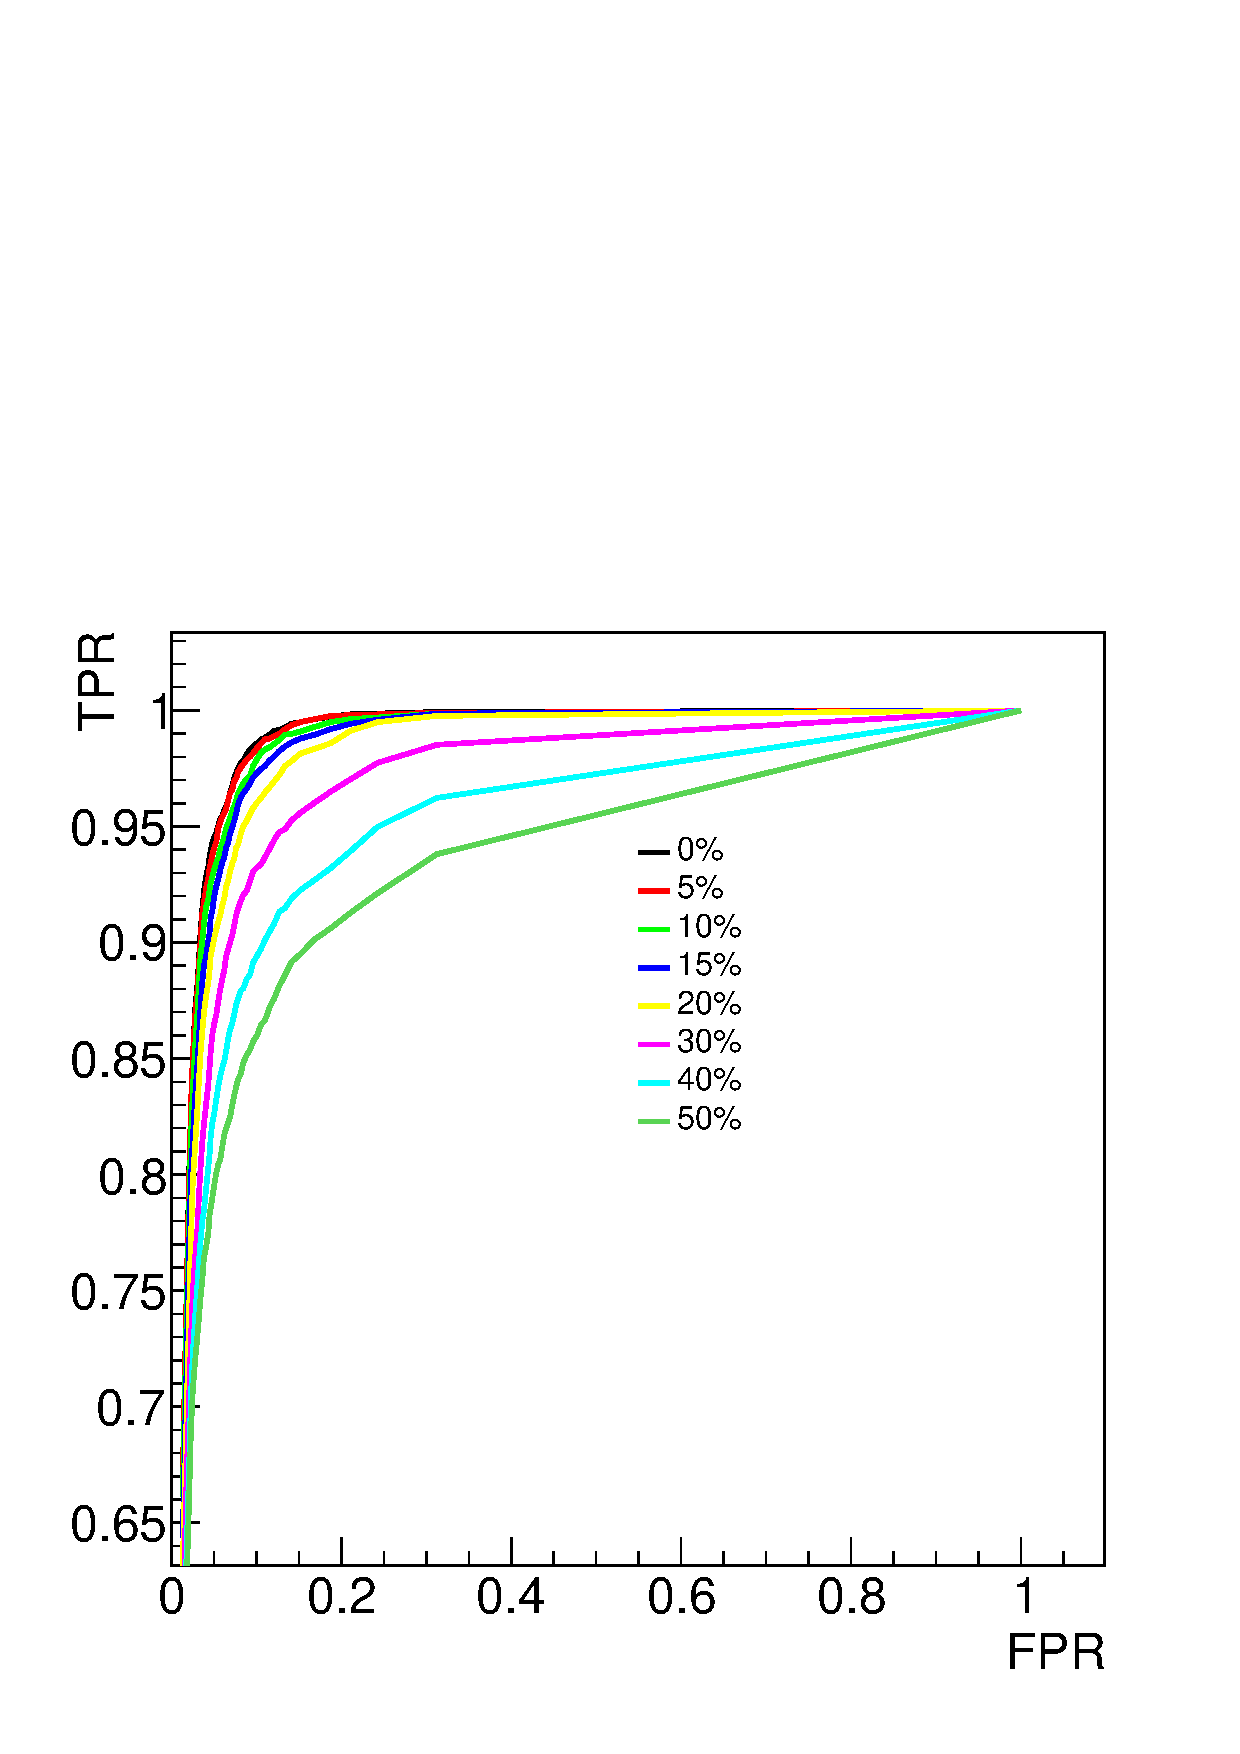
\includegraphics[page=1,width=\linewidth]{/home/kpapad/UG_thesis/Thesis/Bdt/src/WPhiJets_M200M100300_ROCs.pdf}
\caption{}
\label{subfig:SmearingROC}
\end{subfigure}
\begin{subfigure}{0.49\textwidth}
\centering
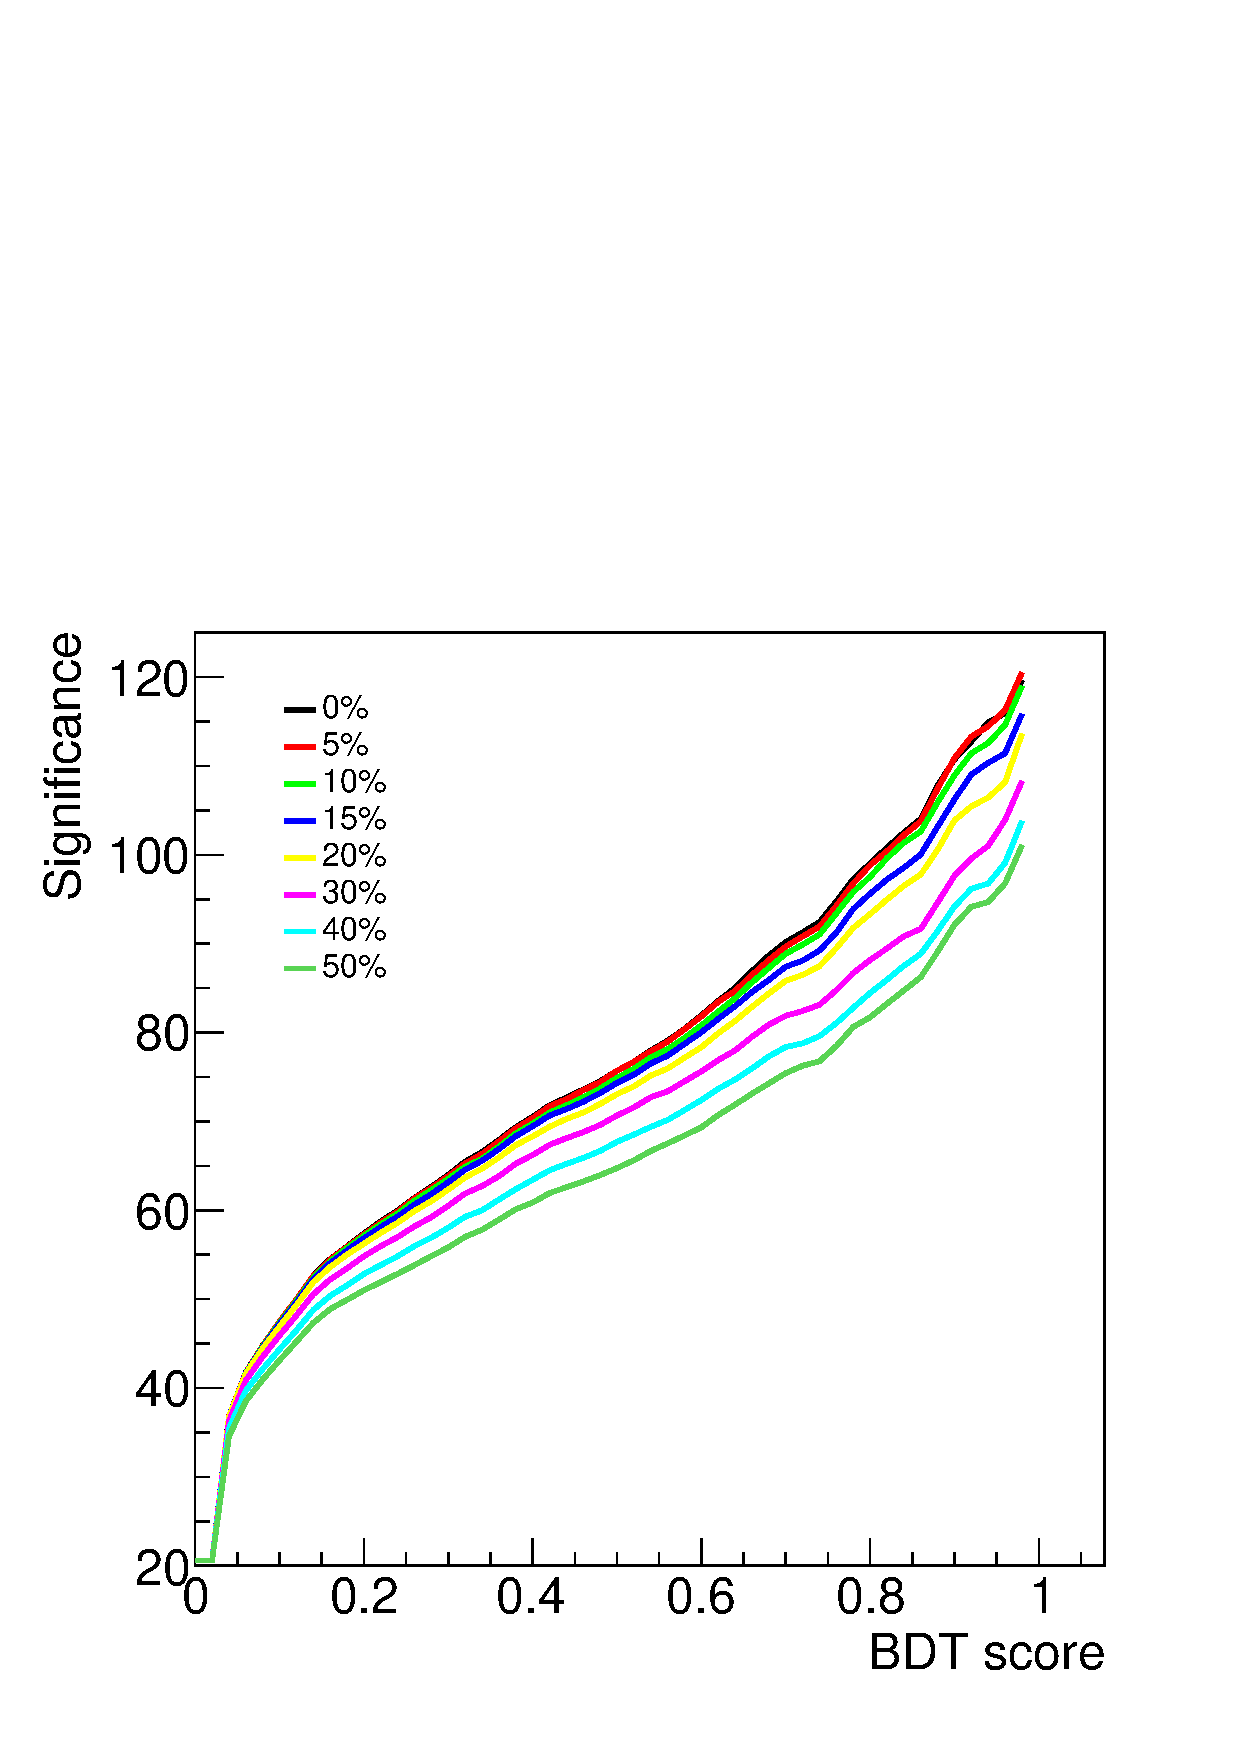
\includegraphics[page=1,width=\linewidth]{/home/kpapad/UG_thesis/Thesis/Bdt/src/WPhiJets_M200M100300_Significance.pdf}
\caption{}
\label{subfig:SigScan}
\end{subfigure}
\caption{a: Summary of the ROC curves for the performance of the model on the data for each smearing case. b: Significances calculated across the BDT score range for the smearing cases of Table \ref{table:Smearings}. The way that these curves are made is analogous to the calculation of the ROC curve.}
\end{figure}

To find the optimal BDT score to place the cut, the whole BDT score range is scanned, and the significance is evaluated in the range [c,1], \(\forall c\in[0,0.98]\) with step size 0.02, same as the bin width of the BDT score histogram(it is pointless to calculate the significance at a single point since it will be 0). The scan of significance for every case of smearing is illustrated in figure \ref{subfig:SigScan}.

Looking at the plot, the cut that gives the best significance is c = 0.98 (the region will be [0.98,1]). Moreover, it is of interest to consider a wider region as well, for the reason that more signal is accepted despite the rejection of less background. To make this argument a bit clearer, let us consider figure \ref{fig:BDTplot}a. At BDT score \textasciitilde{} 7 and onwards, the amount of background events in each bin remains somewhat constant (within statistical fluctuations) while the signal events increase rapidly. It is therefore interesting for our analysis to see how this behavior reflects on the evolution of significance for the various cases of smearing. Looking at figure \ref{subfig:SigScan} again, we conclude that a cut at c = 0.86 is good enough for our purpose.

The results can be seen in Figure \ref{fig:SigEvolBDT} which compares the evolution, in terms of smearing percentage, of the significance for the cuts c = 0.98 and c = 0.86. Table \ref{table:SigBkgBDT} presents the amount of signal and background events present for the two cuts.

\begin{figure}[h!]
\centering
\includegraphics[page=2,width=0.5\textwidth]{/home/kpapad/UG_thesis/Thesis/Bdt/src/WPhiJets_M200M100300_Significance.pdf}
\caption{Evolution of significance for the smearing cases of table \ref{table:Smearings}. }
\label{fig:SigEvolBDT}
\end{figure}


\begin{table}[ht]
\centering
\begin{tabular}{|p{2cm}|p{3cm}|p{3cm}|p{3cm}|p{3cm}|}
 \hline
Smearing \%  & No. Sig. Events at BDT cut = 0.86 & No. Bkg.Events at BDT cut = 0.86 & No. Sig. Events at BDT cut = 0.98 & No. Bkg.Events at BDT cut = 0.98  \\
\hline
0 & 2622.0 & 635.0 & 1977.0 & 273.0 \\
5 & 2615.0 & 635.0 & 1991.0  & 273.0 \\
10 & 2586.0 & 635.0 & 1966.0 & 273.0 \\
15 & 2521.0 & 635.0 & 1914.0 & 273.0 \\
20 & 2464.0 & 635.0 & 1877.0 & 273.0 \\
30 & 2310.0 & 635.0 & 1789.0 & 273.0 \\
40 & 2239.0 & 635.0 & 1715.0 & 273.0 \\
50 & 2173.0 & 635.0 & 1670.0 & 273.0 \\
 \hline
\end{tabular}
\caption{Signal and background events at BDT cut 0.86 and 0.98 for different smearing percentages.}
\label{table:SigBkgBDT}
\end{table}



\subsection{Analysis Method II: Fit based analysis}
\label{sec:org82057fb}
